\documentclass[11.5pt]{sig-alternate} % sets document style to sig-alternate
% packages
% typesetting
%\usepackage{dirtytalk} % typset quotations easier (\say{stuff})
\usepackage{hanging} % hanging paragraphs
\usepackage[defaultlines=3,all]{nowidow} % avoid widows
\usepackage[pdfpagelabels=false]{hyperref} % produce hypertext links, includes backref and nameref
\usepackage{xurl} % defines url linebreaks, loads url package
\usepackage{microtype}
%\usepackage[super]{nth} % easily create superscript ordinal numbers with \nth{x}
%\usepackage{textcomp}
%\newcommand{\texttildemid}{\raisebox{0.4ex}{\texttildelow}}
% layout
\usepackage{enumitem} % control layout of itemize, enumerate, description
\usepackage{fancyhdr} % control page headers and footers
\usepackage{float} % improved interface for floating objects
%\usepackage{multicol} % intermix single and multiple column pages
% language
\usepackage[utf8]{inputenc} % accept different input encodings
\usepackage[english]{babel} % multilanguage support
% misc
\usepackage{graphicx} % builds upon graphics package, \includegraphics
%\usepackage{lastpage} % reference number of pages
%\usepackage{comment} % exclude portions of text (?)
\usepackage{xcolor} % color extensions
\usepackage[backend=biber, style=apa]{biblatex} % sophisticated bibliographies % necessary for HTML to display author info and date on abstract page
\usepackage{csquotes} % advanced quotations, makes biblatex happy
\usepackage{authblk} % support for footnote style author/affiliation
% tables and figures
\usepackage{tabularray}
%\usepackage{array} % extend array and tabular environments
\usepackage{caption} % customize captions in figures and tables (rotating captions, sideways captions, etc)
%\usepackage{cuted} % allow mixing of \onecolumn and \twocolumn on same page
\usepackage{multirow} % create tabular cells spanning multiple rows
%\usepackage{subfigure} % deprecated, support for manipulation of small figures
%\usepackage{tabularx} % extension of tabular with column designator "x", creates paragraph-like column whose width automatically expands
%\usepackage{wrapfig} % allows figures or tables to have text wrapped around them
%\usepackage{booktabs} % better rules
% dummy text
%\usepackage{blindtext} % blind text dummy text
%\usepackage{kantlipsum} % Kant style dummy text
\usepackage{lipsum} %lorem ipsum dummy text
% other helpful packages may be booktabs, longtable, longtabu, microtype

\pagestyle{fancy} % sets pagestyle to fancy for fancy headers and footers

% header and footer
% modern way to set header image
\renewcommand{\headrulewidth}{0pt} % defines thickness of line under header
\renewcommand{\footrulewidth}{0pt} % defines thickness of line above header
\setlength\headheight{80.0pt} % sets height between top margin and header image, effectively moves page contents down
\addtolength{\textheight}{-80.0pt} % seems to affect the lower height. maybe only works properly if footer numbers enabled?
\fancyhf{}
\fancyhead[CE, CO]{
\includegraphics[width=\textwidth]{headerImage.png}}
% footer
%\fancyfoot[LE,LO]{Article Title Here \\ DOI: }% left footer article title and doi
%\fancyfoot[CE,CO]{{}} % center footer empty
%\fancyfoot[RE,RO]{\thepage} % right footer page numbers
%\pagenumbering{arabic} % arabic (1, 2, 3) numbering in footer

\hypersetup{colorlinks=true,urlcolor=blue} % sets link color to blue
\urlstyle{same} % sets url typeface to same as rest of text

% set caption and figure to italics, label bold, left align captions, does not transfer to HTML
\captionsetup{labelfont=bf, font={large, it}, justification=raggedright, singlelinecheck=false}
\renewcommand\theContinuedFloat{\alph{ContinuedFloat}}

%this next bit is confusing, but essentially changes the width of the abstract. Seems to have been copied from this https://tex.stackexchange.com/questions/151583/how-to-adjust-the-width-of-abstract
\let\oldabstract\abstract
\let\oldendabstract\endabstract
\makeatletter %changes @ catcode to enable modification (in parsep)
\renewenvironment{abstract} %alters the abstract environment
{\renewenvironment{quotation}%
               {\list{}{\addtolength{\leftmargin}{1em} % change this value to add or remove length to the the default ?
                        \listparindent 1.5em%
                        \itemindent    \listparindent%
                        \rightmargin   \leftmargin%
                        \parsep        \z@ \@plus\p@}%
                \item\relax}%
               {\endlist}%
\oldabstract}
{\oldendabstract}
\makeatother %changes @ catcode to disable modification

% checks
% italics
% links -
% dashes -
% tildes -
\begin{document}

\title{A Qualitative Study on How Students with Visual Impairments Perceive Environmental Issues}

\author[1]{\large \color{blue}Mustafa Ürey}
\author[1]{\large \color{blue}Maşide Güler}
\affil[1]{Trabzon University}

\toappear{}
%% ABSTRACT
\maketitle
\begin{@twocolumnfalse} 
\begin{abstract}
\item 
\textit {Although there is a growing emphasis on determining how people perceive environmental issues, the studies composed of functioning members of society who happen to have visual impairments are still scarce. The scope of this current paper is aimed at revealing the environmental issue perceptions of middle school students with such conditions. As a part of a large-scale study, this paper presents qualitative data gathered from a well-structured interview protocol. The participants of the study were fifteen Turks from different regions who fell into the aforementioned group. In order to analyse the data, a content analysis technique has been adopted. The results of the study show that they were generally aware of the environment, the environmental problems, the causes of environmental problems, and the effects and remedies of the environmental problems. However, they were not able to relate these problems to their immediate surroundings, and instead carry them to the global dimension.}
\\ \\
Keywords:  environmental issues, visual impairments, middle school students
\end{abstract}
\end{@twocolumnfalse}

%% AUTHOR INFORMATION

\textbf{*Corresponding Author, Maşide Güler}\\
\href{mailto: masidedogan@gmail.com }{(masidedogan@gmail.com)} \\
\textit{Submitted Jun 4 2018 }\\
\textit{Accepted Jul 2 2018} \\
\textit{Published online August 28th, 2018} \\
\textit{DOI:10.14448/jsesd.10.0002} \\
\pagebreak
\clearpage

\begin{large}
\section*{INTRODUCTION}

Although the number of studies related to people with disabilities in general, and those with visual impairments in specific, have emerged in Turkish education literature during recent years, the number of studies are unfortunately not at a desired level. One of the most known symposiums, the 12th National Congress of Science and Mathematics Education, which was held in Turkey in 2016, showed that only four presentations took place related to students with visual impairments among 1,000 proceedings. Considering there are 253 million people  with vision impairments in the world (The World Health Organization [WHO], 2017), the equal education of those people becomes crucial, necessitating many routes for access. 

WHO (2009) divided vision quality into four categories: normal vision, mild vision loss (partial vision), significant vision loss (low vision) and no vision (total blindness). Individuals who have significant vision loss cannot even read with regular text accessories (glasses, lenses, etc.). With total blindness, it is not possible to read at all. Such individuals can read and write with the Braille alphabet, or get help from electronic devices (Cox \& Dykes, 2001). Despite these challenges, they are as qualified as normal-sighted individuals in acquiring skills in educational programs (Kumar, Ramasamy, \& Stefanich, 2001), as well as being developed as individuals who have full cognitive abilities (Jones, Minogue, Oppewal, Cook, \& Broadwell, 2006). 

It is known that some teachers have some prejudices about how learning works for people who are blind (Stefanich \& Norman, 1996), although it has been stated that they are predisposed to learning as normal individuals. However, given the individual differences that people have, it is necessary that, in accordance with the principle of equality in education, those with disabilities are not pushed to the background due to the extra factor. Indeed, since the level of education is directly related to the standards of life of the individual, it is necessary that individuals who have any impairments are not abstracted from the educational experience because of them (Cavkaytar, 2012). They should not be ignored in educational research. The Turkish ministry of education has signed an agreement via the care of the United Nations in 2009, and the first paragraph of Article 24, is as follows:

\begin{itemize}
    \item “States Parties recognize the right of education for persons with disabilities and provide lifelong learning and integration of the system of education on an equal basis and non-discriminatory basis, in an integrative way, at all levels. The following objectives should be observed for this:
\begin{enumerate} [label=\alph*.]
    \item  Strengthening the full development of the human potential, the sense of dignity and value, and respect for human rights, fundamental freedoms and human diversity;
    \item  Your disability; ensuring that their personality, their talents, their creativity, their mental and physical skills are developed at the highest level of potential;
    \item  Ensuring participation of disabled people in a free society (Official Gazette, 2006).”
\end{enumerate}
\end{itemize}

The development of individual talents and creativity is possible, first of all, with content which mentally activates those abilities. One of these subjects is science (Yilmaz et al., 2008), in which individuals can acquire different information by establishing interrelationships between concepts through their achievements, and to find and test them in hypotheses. Science is a research and thinking path that is based on continuous inquiry, as well as experimental criteria and logical thinking (TTKB, 2006). A Science and Technology course (Ayvacı, 2012), which aims to educate literate individuals, was expressed as a composition of skills, attitudes, values, understandings and knowledge about science that promotes critical thinking skills. Those skills must be possessed in order to sustain the curiosity about the environment and the world.

When the curriculum is examined, it appears that 7 dimensions have been put into the foreground in order to train science literate individuals. These are:

 \begin{enumerate}
     \item The nature of science and technology
     \item Key science concepts
     \item Scientific process skills
     \item Scientific/Technological/Societal/Environmental relations
     \item Scientific and technical psychomotor skills
     \item Some values which constitute the nature of science
     \item Some attitudes and values towards science (TTKB, 2006)
 \end{enumerate}

Scientific/Technological/Societal/Environmental relations, which take place in the above dimensions and have an important place among the general aims of the science course, should not only recognize the interactions between those factors but also recognize the environmental problems and take responsibility for them and make decisions (TTKB, 2006).

In the literature, there are numerous studies on science teachings that are carried out on individuals with visual impairments (e.g. Sözbilir et al., 2015; Supalo, Isaacson \& Lombardi, 2013; Tezcan, 2012; Tuncer \& Kahveci, 2009; Ünlü, Pehlivan \& Tarhan, 2010; Winchatz \& Riccobono, 2008). However, there are a limited number of studies evaluating their environmental awareness or awareness of environmental problems (Maji, 2014; Sengupta, Banerjee \& Maji, 2009). This current study attempted to investigate how students with visual impairments perceive environmental issues. Briefly, the research questions are the following:

\begin{itemize}
    \item What do the students with visual impairments think about the existing environmental issues?
    \item What do the students with visual impairments think about the reasons for those issues?
\end{itemize}

\section*{METHOD}
This current study aimed to examine how middle school students with visual impairments perceive environmental issues, and what they think about the causes of these issues. It is  descriptive research as it aims to present a picture of the current situation in the study. On the other hand, it can be said that this study is a special case method, since it has been conducted with a limited sample (Creswell \& Clark, 2007). As part of a large-scale study, this research presented the views of students with visual impairments on environmental issues and their thoughts about those issues. In the study conducted by the main workshop with 87 participants, five students from each group who got the highest score of anthropocentric, ecocentric and antipathetic opinions were identified, and interviews were conducted with a total of 15 students on the basis of volunteerism. This paper presents data from those interviews. The background of the participants is as given in Table 1.

\begin{table*}[th]
\caption{Characteristics of the participants}
\begin{tabular}{ccccc}
\hline
\textbf{Code} & \textbf{Gender} & \textbf{Grade} & \textbf{Level of Blindness} & \textbf{Views toward environment} \\ \hline
S\textsubscript{24} & Male & 8th & Totally Blind & Ecocentric \\ \hline
S\textsubscript{29} & Female & 8th & Totally Blind & Ecocentric \\ \hline
S\textsubscript{30} & Male & 7th & Visual Impairment & Ecocentric \\ \hline
S\textsubscript{31} & Male & 7th & Visual Impairment & Ecocentric \\ \hline
S\textsubscript{15} & Male & 6th & Totally Blind & Ecocentric \\ \hline
S\textsubscript{12} & Female & 8th & Totally Blind & Anthropocentric \\ \hline
S\textsubscript{1} & Male & 6th & Visual Impairment & Anthropocentric \\ \hline
S\textsubscript{5} & Male & 8th & Visual Impairment & Anthropocentric \\ \hline
S\textsubscript{20} & Female & 5th & Totally Blind & Anthropocentric \\ \hline
S\textsubscript{22} & Female & 6th & Visual Impairment & Antipathetic \\ \hline
S\textsubscript{21} & Female & 5th & Visual Impairment & Antipathetic \\ \hline
S\textsubscript{14} & Male & 7th & Totally Blind & Antipathetic \\ \hline
S\textsubscript{19} & Female & 5th & Visual Impairment & Antipathetic \\ \hline
S\textsubscript{3} & Female & 6th & Visual Impairment & Antipathetic \\ \hline
S\textsubscript{13} & Male & 7th & Totally Blind & Antipathetic \\ \hline
\end{tabular}
\end{table*}

\subsection*{Data Collection Tool}

In the study, "structured interviews" were carried out on students with visual impairments selected through purposeful sampling so that the individuals could voice their in-depth views of environmental issues. A structured interview is a type of interview in which participants are asked how to ask questions beforehand, and the interview plan is followed (Karasar, 2005). In other words, it is the interview technique plan which is the most detailed in terms of what kind of questions are asked and in what way, and what data is gathered and what is the most detailed data collection form (Çepni, 2010). Before the interview questions were determined, the literature about perception of environment was searched, and the interview questions in the field-related studies were examined. After reviewing the literature and interview questions, informal interviews were held with two students with visual impairments to decide which interview questions should be used. This approach was used with the aim of gathering rich and sufficient data, and to facilitate the comparisons and analyses while discussing and presenting the existing information about the subject through the informal interviews (Büyüköztürk, Kılıç-Çakmak, Akgün, Karadeniz, \& Demirel, 2013; Çepni, 2010). 

\subsection*{Data Analysis}

A content analysis was conducted in the analysis of the interview data. Within the scope of this study, the voice records were taken with the permission of the participants, and the data was transferred to an electronic media program, the data in the electronic media then was transcripted and converted into written documents. The written format of the interviews was coded using NVivo, which is a useful model-building tool for qualitative research (Richards, 1999), and the conclusions made from the encodings created appropriate themes for the interview questions. The themes were created in the direction of the students’ perspective, and the codes obtained were placed under the relevant themes. Concept maps were created from the obtained themes and codes to facilitate the work of the reader, and thus, the tables were created by displaying the opinions of each participant about each research question. Miles and Huberman's (1994) Reliability = Opinion Alliance / (Opinion Alliance + Opinion Separation) formulaic assessment of their agreement levels towards such questions was calculated to be 0.86, and disagreements were discussed until reaching a consensus between the researchers. Therefore, one can say that the reliability of the paper has been provided.

\section*{RESULTS}

This part of the paper showed conceptual networks about what the perceptions of the students with visual impairments on the environmental issues were, and the reasons for these environmental problems from their perspectives. In this regard, themes and codes were presented with respect to the data gathered from the interviews. 

\subsection*{Perceptions of Living Environmental Problems}

Ten different themes and 51 different codes were obtained related to this theme as a result of the thoughts of what environmental problems of the middle school students with the aforementioned conditions experienced. These included: the problems of environmental resources and nutrition, urbanization problems, agricultural problems, waste problems, air pollution, water pollution, soil pollution, noise pollution, solid waste pollution and environmental education problems. Figure 1 represents the codes related to the use of natural resources and nutrition, and urbanization problems. 
 
\begin{figure*}[tp]
    \centering
    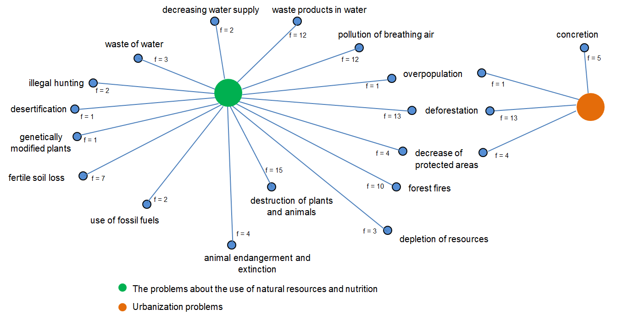
\includegraphics[width=1\textwidth]{Fig1.png}
    \caption{Problems about the use of natural resources and nutrition, and urbanization }
\end{figure*}

As can be seen in Figure 1, the relevant views of students with visual impairments spanned a wide-range of codes. The most common of these codes was the destruction of plants and animals. The decline in the number of trees, deforestation, was the most frequently repeated code. The natural water’s pollution and air pollution were other important points emphasized by them. Some of these codes were specified with this theme (urbanization) because they were related to the results of urbanization. Concrete, on the other hand was one of the most mentioned issues among urbanization problems. The sequence from an interview conducted to a student about the subject was as follows:

S\textsubscript{15}: “…Future resources are exhausted. For example, our waters are exhausted because we hurt the environment, and our waters are polluted because we throw garbage into the sea. Water is the main source of our life. For example, when animals kill or hunt animals that are prohibited from hunting, animals become extinct…”

When the answer given by the student interviewed above is examined, it is seen that the student is paying attention to the depletion of water resources, destruction of animals and illegal hunting. A followup on the conducted interview with a different student was as follows:

S\textsubscript{5}: “….We consume products with GMOs. [The concept of a] GMO (genetically-modified organism) is something about growing fruits anytime [which] normally grow a certain season of the year.”

It is seen that that student’s response attracted attention to the genetically modified plants, unlike the other students’, and expressed these plants as environmental problems. Another interview data which is related to urbanization and the use of natural resources and nutrition was as follows: 

S\textsubscript{12}: “The more people [who] construct houses and buildings, the more [the green areas diappear]. Too many houses are being built, and [their number] is increasing day by day. Trees are being cut in Turkey while we should grow them.”

When this answer is examined, it is seen that the student emphasizes deforestation and emphasizes the reduction of green areas, so that attention is paid to the construction rate of buildings while tree plantings are decreasing. The codes obtained from the agricultural problems and soil pollution theme is presented in Figure 2.
 
\begin{figure*}[tp]
    \centering
    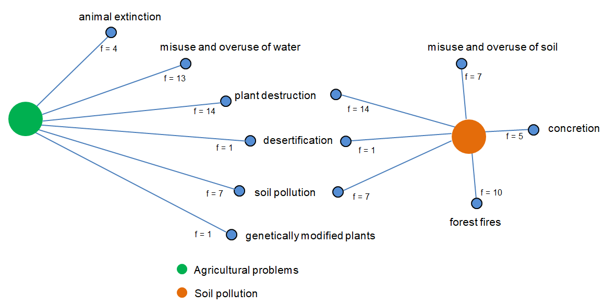
\includegraphics[width=1\textwidth]{Fig2.png}
    \caption{The codes regarding agricultural problems and soil pollution}
\end{figure*}

When Figure 2 is examined, it is seen that the participants stated destroying plants, soil pollution and desertification problems in relation to both soil pollution and agricultural issues. Among them, the most repetitive code has been the desturction of plants, which is expressed by almost all of the participants. In connection to the agricultural problems theme, the misuse and overuse of water was mentioned by most of the students. Animal extinction and genetically modified plants were other topics which students mentioned.  On the other hand, in terms of soil pollution, the “forest fires” code was stated by two out of three of the students. Concretion and the misuse and overuse of soil were the other codes. As for other themes, waste problems and water pollution were extracted from the interview. The themes and codes belonging to those themes are presented in Figure 3.

\begin{figure}[tp]
    \centering
    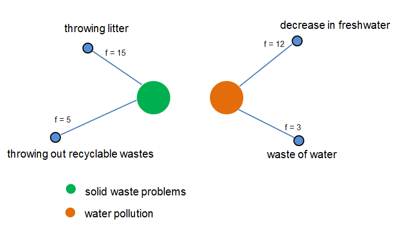
\includegraphics[width=1\linewidth]{Fig3.png}
    \caption{The codes regarding to solid waste problems and water pollution}
\end{figure}

As shown in Figure 3, it can be seen that two codes were obtained for each of the themes of waste problems and water pollution. These include littering and throwing out recyclable wastes at one side, and the decrease in fresh water and waste of water at the other side. As one of the waste problems, all participants emphasized littering in nature. An interview session with S30 contained their following idea:

S\textsubscript{30}: “People are throwing the [empty] bottle[s] of water they [don’t need], the food they [could have eaten], and [used] chewing gum around. The birds think that the gum is food, and they try to eat it, then they choke and die. Those plastic bottles do not disappear for thousands of years [in] nature.” 

\begin{figure*}[tp]
    \centering
    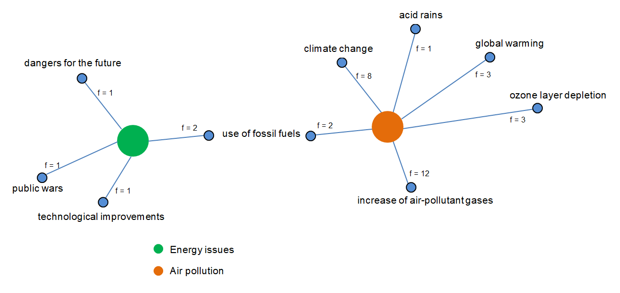
\includegraphics[width=1\textwidth]{Fig4.png}
    \caption{The codes of energy issues and air pollution themes}
\end{figure*}

The response of S\textsubscript{30} draws attention to waste problems by giving a current example of how people pollute the environment. Specifically, five of those students mentioned throwing out recyclable wastes. In relation to their daily experiences, students mostly referred to “paper” as recyclable waste. The other two themes were energy issues and air pollution, consisting of one common code and a total of nine codes (see Figure 4). 

For the theme of energy issues, it was obtained that technological improvements, the dangers for the future, and public wars between countries were codes, while climate change, acid rain, global warming, the thinning of the ozone layer, and increases in air-pollutants were acquired for the theme of air pollution. Commonly with two of the themes, the use of fossil fuels was indicated by the participants. When the codes are examined, it is seen that many of the students referred to the increase of air-polluting gases as air pollution. A snippet of an interview session with S20 is presented below.

S\textsubscript{20}: “…when you use fossil fuels, toxic gases come out. Fossil fuels come from underground sources, such as coal [and] oil, and [cause] air pollution.”

When the response is examined, it can be said that the student is aware of the effects of consuming fossil fuels and their effects on nature. When the responses of the other students are examined, similar ideas are encountered. The common emphasis that students have made here is the characteristics of the polluting gases and how they affect the environment. It is also seen that the effects of human influences on environmental pollution is the forerunner in their perspective. Surprisingly, climate change and global warming codes were highlighted by the students frequently. For instance, S14 student’s code-based views are given as:

S\textsubscript{14}: “…... air is getting warmer due to air pollution; global warming is happening and seasons are shifting, so climates are changing ...”

Finally, two more themes extracted from student interviews were noise pollution and environmental education problems. The relevant themes and codes are presented in Figure 5.
 
\begin{figure}[h]
    \centering
    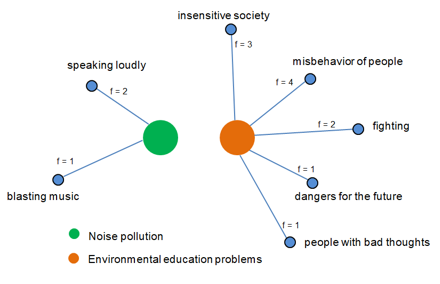
\includegraphics[width=1\linewidth]{Fig5.png}
    \caption{The codes of noise pollution and environmental education problems}
\end{figure}

According to Figure 5, it can be said that the codes obtained from both themes are less in the noise pollution dimension than the pollutions in the previous ones. As a matter of fact, only the “speaking loudly” and “blasting music” codes were included, and the total frequency for them was 3. On the other hand, it was also pleasing to obtain the theme of environmental education problems. As far as the findings here are concerned, it is necessary to have an education about it, as mentioned in the discussion section. It is also worth mentioning that this need includes students with visual impairments. 

\subsection*{Perceptions of the Causes of Environmental Problems}

Table 2 shows the themes and codes regarding the causes of environmental problems which students with visual impairments are also aware of.

\begin{table*}[th]
\caption{Themes and codes for the causes of environmental problems}
\begin{tabular}{cccc}
\hline
\textbf{Themes} & \textbf{Sub-themes} & \textbf{Main Codes} & \textbf{Codes} \\ \hline
\multirow{6}{=}{Anthropocentric} & Directly anthropocentric & Knowledge, susceptibility, awareness & Forest fires, glass wasting, deforestation, leaving the water on/wasting and overconsuming water, illegal hunting, gas emissions caused by people, killing animals \\
\cline{2-4}
 & \multirow{5}{=}Indirectly anthropocentric & Industry & Released fumes, factory wastes, heating the earth \\
\cline{3-4}
 & & Technology & Improvements of technology, technological wastes \\
\cline{3-4}
 & & Urbanization & Domestic wastes, making more buildings than necessary, overpopulation, constructing malls and factories, cutting down trees \\
\cline{3-4}
 & & Tourism & Building more houses and hotels, polluting the water \\
\cline{3-4}
 & & Traffic & Air pollution, exhaust fumes, increases in the number of vehicles, over-heating of the earth \\ \hline
Non-anthropocentric & & Natural Disasters & Excessive erosion, landslides, avalanches, earthquake, flooding \\ \hline
\end{tabular}
\end{table*}

When we examine Table 2, which shows the reasons of living environmental problems in terms of the students’ opinions, it is seen that two themes regarding them are human-centered environmental problems (anthropocentric) and non-human centered environmental problems (non-anthropocentric), and from these themes, direct anthropocentric and indirect anthropocentric sub-themes were extracted. In relation to the anthropocentric sub-theme, one direct main code was generated, while there were five indirect, anthropocentric main codes. For the non-anthropocentric theme, only one main code was generated. For example, “knowledge, susceptibility, and awareness” was coded as one of the responses given by the students, as in the upcoming excerpt.

S\textsubscript{1}: “People are throwing trash around the street. When people think about themselves and do not think of other living things, for example, the animals become extinct because people make bags, jackets[, etc.] from their skin; [they] earn money by selling animals…”

In this response, in which the direct human impact is apparent, it appears that the student had used expressions of trashing and killing animals. Again, this response, which is related to sensitivity and awareness, is important in order to provide a sample case that is frequently encountered in everyday life. Students with visual impairments have often seen released industrial gases as an example of an indirect anthropocentric pollution source. Besides, the code for cutting down trees, which is located under urbanisation, is one of the frequently repeated codes. The two sample responses are as follows:

S\textsubscript{14}: “... fumes from factory floors, [and] coal fumes from workplaces and mines are polluting the air. Factory wastes also cause water pollution ...”

S\textsubscript{29}: “…many trees are being cut [down] and shopping malls are being built; I am very against this. For example, people in shopping malls say that I am [enabled to interact more] with people [because of it], but if they do not cut those trees [down] and people stay in green places, maybe they will find more peace…”

Finally, responses to natural disasters under the non-anthropocentric theme included codes tied to excessive erosion, landslides, avalanches, earthquakes, and flooding. 

\section*{DISCUSSION AND CONCLUSION}

This paper aimed to determine the perceptions of students with visual impairments on environmental issues, and their thoughts on the reasons for them. Interviews with such students in this context revealed important clues on how they perceive both these issues and their sources. First of all, the words that students used mostly consisted of concepts such as plants, animals, nature, soil, and water belonging to the natural environment, in addition to artificial environments, such as homes, factories, hotels, and shopping malls. From this point of view, it appears that they have included elements of the artificial and socio-economic environment to depict a limitation of their living conditions from the natural environment. It is striking that the interviewed students with visual impairments placed more importance on the concept of plants, animals, and humans being components of natural environments. In this case, it can be concluded that for those students, plants were conceptually more important to them in comparison to students with normal vision. In addition, the concept of humans being able to live harmoniously with plants and animals was also frequently mentioned, which supports the expression that human beings are a part of nature, too. On the other hand, it was seen that the students additionally included inanimate elements, which are elements of an artificial and socio-cultural environment created by humans apart from the natural environment, and in one bounded by their own living quarters. Similarly, Yardımcı and Bağcı-Kılıç (2010) found that 8th grade primary school students perceive the environment as a place which consists of living and non-living elements. They also found that the children dominantly acknowledged plants more than animals or humans when confronted with the state of the environment. Littledyke’s (2004) report can be interpreted to say the fact that most primary school students expressed the environment to be made up of living creatures such as plants, animals, and human beings, and that the younger students perceived the environment more as living things. In that study, based on the students’ interpretations, it can be interpreted that all of those students generally perceived the environment more as living things.

Findings from student interviews on what environmental problems are associated with concluded that the included students with visual impairments mostly concentrated on the use of natural resources and problems such as diet-based impacts, urbanization, energy consumption, agriculture, waste, pollution, and environmental education. While those students focused on air, water, soil, and noise pollution as pollution problems, they did not actively consider radioactive and light pollution forms during the sessions, as mentioned before. In addition, it is striking that they perceived the problem arising from the deficiencies in environmental education as an environmental problem, as is pointed out in the literature.  Also, they were aware of the above mentioned environmental problems, especially air pollution, forest fires, deforestation, water pollution, and so on. This supports the findings of those students with visual impairments to be, directly or indirectly, main fighters against environmental problems. These findings showed that the vast majority of the students expressed various environmental problems and that they knew about not all, but most of the issues. The issues they indicated were within their immediate surroundings, or limited to what they have heard. For instance, they rarely mentioned the thinning of the ozone layer or acid rain, and never touched some kinds of issues, such as radioactive pollution. One of the causes of this situation may be that the students were young. This claim was supported by Alerby’s study (2000), which revealed that young children expressed environmental issues from their immediate environment, referring to wastes, while older children reported environmental problems, such as global warming, the greenhouse effect, and the thinning of the ozone layer, which are not directly in close proximity to them.

According to the students’ opinions on the causes of environmental problems, both direct and indirect human effects were the most frequently repeated responses. Considering these results, one can say that those students with visual impairments were aware of the human factor as the primary cause of environmental problems, and how people are overusing nature in favor of their own interests. Similarly, Yardımcı and Bağcı-Kılıç (2010) noted that when asking children what kind of environment they wanted, they asked for an environment with the least people, or an environment where there were no negative human effects. As can be seen in this study, students are aware of the negative effects of people, even if they have visual impairments. 

\end{large}
\clearpage 
\section*{REFERENCES}\par 

\leftskip 0.25in
\parindent -0.25in 

Alerby, E. (2000). A way of visualizing children’s and young people’s thoughts about the environment: A study of drawings. \textit{Environmental Education Research, 6}(3), 205–222.

Ayvacı, H.Ş. (2012). \textit{Teknolojik proje tasarımı}. Ankara: PegemA.

Büyüköztürk, Ş., Kılıç Çakmak, E., Akgün, Ö.E., Karadeniz, Ş., \& Demirel, F. (2013). 	\textit{Bilimsel araştırma yöntemleri} [Scientific research methods] (15. Baskı). Ankara: Pegem Akademi Yayınları.

Cavkaytar, A. (2012). Özel eğitime gereksinimi olan öğrenciler ve özel eğitim. İbrahim, D. (Ed.), \textit{Özel eğitime gereksinimi olan öğrenciler ve özel eğitim}. ss. 1-28). Ankara: Pegem Akademi.

Cox, P. R., \& Dykes, M. K. (2001). Effective classroom adaptations for students with visual impairments. \textit{Teaching Exceptional Children, 33}(6), 68-74.

Creswell, J. W., \& Clark, V. L. P. (2007). \textit{Designing and conducting mixed methods research}. Thousand Oaks, CA, US: Sage Publications, Inc.

Çepni, S. (2010). \textit{Araştırma ve proje çalışmalarına giriş} (Geliştirilmiş 5. Baskı) Trabzon: Celepler Matbaacılık.

Jones, M. G., Minogue, J., Oppewal, T., Cook, M. P., \& Broadwell, B. (2006). Visualizing without vision at the microscale: Students with visual impairments explore cells with touch. \textit{Journal of Science Education and Technology, 15}(5-6), 345-351.

Karasar, N. (2011). \textit{Bilimsel araştırma yöntemi} (22.Baskı). Ankara: Nobel Yayıncılık. 

Kumar, D. D., Ramasamy, R., \& Stefanich, G. P. (2001). Science for students with visual impairments: Teaching suggestions and policy implications for secondary educators. \textit{Electronic Journal of Science Education, 53}. Retrieved from \url{http://ejse.southwestern.edu/article/viewArticle/7658/5425} [November 10, 2016]. 

Littledyke, M. (2004) Primary children’s views on science and environmental issues: examples of environmental cognitive and moral development. \textit{Environmental Education Research, 10}(2), 217-235.

Maji, P. K. (2014). Environment related behaviour of the students who are visually impaired. \textit{Journal of Education and Human Development, 3}(2), 793-808.

Miles, M. B. \& Huberman, A. M. (1994). \textit{Qualitative data analysis} (2. baskı). Thousand Oaks, CA: Sage Publications.

Official Gazette (2009). Engellilerin haklarına ilişkin milletlerarası sözleşme [United Nations Convention on the Rights of Persons with Disabilities]. Retrieved from tarihinde \url{http://www.resmigazete.gov.tr/eskiler/2009/07/20090714-1.htm}  [September 30, 2016].

Richards, L. (1999). Data alive! The thinking behind NVivo. \textit{Qualitative Health Research, 9}(3), 412-428.

Sengupta, M., Banerjee, D., \& Maji, P.K. (2009). Effect of sight and gender on environmental awareness and pro-environmental behaviour amongst school students. \textit{Journal of All India Association for Educational Research, 21}(1), 60-63.

Sözbilir, Ö., Gül, Ş. Okçu, B., Yazıcı, F., Kızılaslan, A., Zorluoğlu, S. L., \& Atilla, G. (2015). Trends in research papers about teaching science to visually impaired students. \textit{Abant İzzet Baysal Üniversitesi Eğitim Fakültesi Dergisi, 15}(1), 218-241.

Stefanich, G. P., \& Norman, K. I. (1996). Teaching science to students with disabilities: Experiences and perceptions of classroom teachers and science educators. Washington , DC: Association for the Education of Teachers in Science.

Supalo, C. A., Isaacson, M. D., \& Lombardi, M. V. (2013). Making hands-on science learning accessible for students who are blind or have low vision. \textit{Journal of Chemical Education, 91}(2), 195-199.

Talim Terbiye Kurulu Başkanlığı [TTKB] (2006). \textit{İlköğretim fen ve teknoloji dersi öğretim programı ve kılavuzu: 6, 7 ve 8. Sınıflar}. Ankara: Devlet Kitapları Müdürlüğü.

Tezcan, C. (2012). \textit{Establishment of mentally retarded children's web-based distance education system: application of mathematics and science courses}. (Unpublished master thesis). Trakya University, Edirne.

The World Health Organization [WHO]. (2009). Visual impairment and blindness. Retrieved from \url{http://www.who.int/mediacentre/factsheets/fs282/en/index}  [September 29, 2016].

The World Health Organization (WHO) (2017). Blindness and visual impairment. Retrieved from  \url{http://www.who.int/news-room/fact-sheets/detail/blindness-and-visual-impairment} [January 1, 2018]. 

Tuncer, A. T. \& Kahveci, G. (2009). Teaching how to use of concept maps in summarizing texts by usıng peer mediation to 8th grade students with low vision. \textit{Türk Eğitim Bilimleri Dergisi, 7}(4), 853-877.

Ünlü, P., Pehlivan, D., \& Tarhan, H. (2010). The Sight-Impaired High School Students' Opinions About Physics Course. \textit{Gazi Üniversitesi Gazi Eğitim Fakültesi Dergisi, 30}(1), 39-54.

Winchatz, B. B. \& Riccobono, M. A. (2008). Advancing participation of blind students in science, technology, engineering, and math. \textit{Advances in Space Research, 42}(11), 1855-1858.

Yardımcı, E. \& Bağcı-Kılıç, G. (2010). Children’s views of environment and environmental problems. \textit{Elementary Online, 9}(3), 1122-1136.

Yılmaz, F., Atalay, H., Özgül, E., Keleş, Ö., Gürer Kavas, B., Şen, N., ….. Şahin, S.(2008). \textit{İlköğretim fen ve teknoloji ders kitabı}. İstanbul: Milli Eğitim Bakanlığı Devlet Kitapları.

\end{document}